\documentclass[12pt, a4paper]{report}

%% Dansk shizzle
\usepackage[utf8]{inputenc}
\usepackage[T1]{fontenc}
\usepackage[danish]{babel}

%% Sideopsætning
\usepackage{setspace}
\onehalfspacing
\usepackage{fix-cm}
\usepackage[a4paper,margin=2.5cm,headheight=2cm]{geometry}
\usepackage{lastpage}
\usepackage{fancyhdr}
\usepackage{graphicx}
\usepackage{sidecap}
\usepackage{units}
\pagestyle{fancy} %skift til fancy
\fancyhead[L]{Kollegiekontoret}
\fancyhead[R]{\today}
\fancyfoot[L]{SUM2 Projekt}
\fancyfoot[C]{Side \thepage\ af \pageref{LastPage}}
\fancyfoot[R]{Team Awesome}


\setcounter{secnumdepth}{-1}
\title{SUM Projekt - Kollegiekontoret}
\author{Silas Fontain Jakobsen \and Tina Jensen \and Andreas Kristoffersen \and Jannie Gier Larsen \and Erik Holm Sejersen}
\date{21. Maj 2012}

% latex crash course: http://www.haptonstahl.org/latex/

\begin{document}
\begin{titlepage}
\maketitle
\end{titlepage}

\begin{abstract}
\thispagestyle{empty}
Forord
\end{abstract}

\tableofcontents

\chapter{Forundersøgelse}

% SKRIV OM HVAD EN FORUNDERSØGELSE ER

Vi har lært om at bruge MUST-metoden, og det er overordnet denne metode vi vil anvende principper og værktøjer fra i forundersøgelsen. På vores plan under afsnittet metode, kan overskrifter for de begreber vi har arbejdet med ses.

\section{Forberedelse og projektgrundlag}
På vores indledende projektetableringsmøde blev vi enige om projektets omfang og blev enige om, at vi med al sandsynlighed ikke når at levere et færdigt og brugbart produkt indenfor den afsatte tid.

\subsubsection{Baggrund}
Vi har i forbindelse med en stillet eksamensopgave taget kontakt til Kollegiekontoret, da de har et kommende IT projekt med henblik på at få opgraderet deres hjemmeside til udlejning af ungdomsboliger.

\subsubsection{Opgaven og formål}
Vores opgaver består i at afdække Kollegiekontorets behov til en ny hjemmeside, der er tidssvarende og giver potentielle lejere et bedre overblik over deres muligheder for at leje en ungdomsbolig.

\subsubsection{Økonomiske og tekniske rammer}
Der er ikke afsat økonomiske midler til projektet, og vi kan ikke forvente der er mulighed for at tilføje flere ressourcer. Vores tekniske rammer og værktøjer er hvad vi har lært at anvende i studietiden, og der er hverken tid eller penge til større oplæring/kurser.

\subsubsection{Kritiske faktorer}
Det er ikke målet at vi på den afsatte tid når at udvikle et kørende system, og Kollegiekontoret forbereder sig også på at købe systemet af en anden leverandør. Vores mål med projektet er således dels at lære at anvende de lærte begreber og metoder, og dels at vise kollegiekontoret den agile side af udviklingsverdenen i praksis.

\subsection{Organisering}
\subsubsection{Projektets organisering}
Projektgruppen består primært at de fem undertegnede, hvoraf Tina Jensen er valgt som formel leder af gruppen. Kollegiekontorets interesser kan repræsenteres i projektgruppen af Silas F. Jakobsen der er medlem af Kollegiekontorets Forretningsudvalg. Kontakterne der arbejder til dagligt på Kollegiekontoret er informationsmedarbejder Lene Billeskov Jensen og administrationschef Diana Jørgensen. Andreas Kristoffersen er valgt som ansvarlig for versions- og dokumentstyring.
I princippet kunne en formel styregruppe etableres med kontaktpersonerne fra kollegiekontoret, men da dette også er et læringsprojekt vil vi alle gerne være lidt involveret i beslutningsprocesserne, og når hele projektgruppen indgår er det lidt strakt at kalde det en styregruppe.

\subsubsection{Ressourcer}
Uden tildelte økonomiske midler må vi anvende de gratis værktøjer vi kan få fat i, heldigvis er udbudet af gratis værktøjer ganske omfattende. Vi har opsat infrastruktur i form af dokumentstyring og versionskontrol, og vi har de nødvendige udviklingsværktøjer til rådighed.
Til versionsstyring og generel filudveksling har vi valgt at bruge Git. Det er ikke hele teamet der har erfaring med dette værktøj, men grundet dårlige erfaringer med konkurrerende værktøjer ser det ud som om det er det bedste bud.
Til rapporten faldt valget på \LaTeX og Google docs. Google docs fungerer godt når flere skal rette i et dokument på samme tid og \LaTeX er uden sammenligning den bedste måde at håndtere skriftlige dokumenter over en vis størrelse.

\subsubsection{Interessenter}
Vi vurderer, at der på projektet findes følgende relevante og klart definerede interessenter:
\begin{itemize}
\item Kunde: Kollegiekontoret
\item Leverandør: Team Awesome
\item Projektleder: Tina Jensen
\item Slutbrugere: Nuværende og potentielle lejere af ungdomsboliger i Aarhus
\item Udviklere: Team Awesome
\item Testere: Team Awesome
\item Konsulent: Hanne Sommer
\end{itemize}

\begin{figure}[h!]
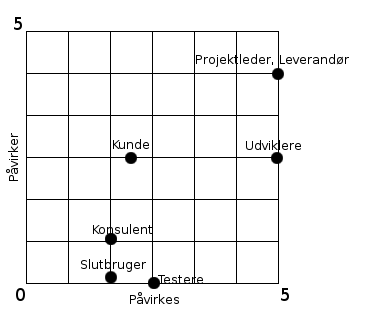
\includegraphics[width=0.5\textwidth]{interessenter}
\caption{Figur, der viser interessenternes indflydelse.}
\end{figure}

\begin{figure}[h!]
  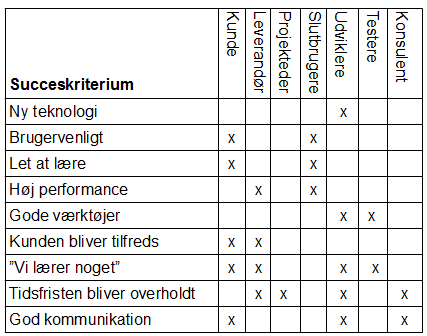
\includegraphics[width=0.5\textwidth]{succeskriterium}
  \caption{Figur, der viserinteressenternes succeskriterier .}
\end{figure}

En mulig konflikt i vores succeskriterier - i og med at der er tale om et skoleprojekt - kan være at vi som studerende har mere fokus på at lære noget, end at levere noget kunden kan bruge og bliver tilfreds med. Udviklingsforløbet er en læringsproces for os, som derfor vil tage længere tid på hver enkelt del end en udvikler fra erhvervslivet, og vi vil lave flere eksperimenter med hvordan produktet skal fungere, som måske ikke er forenlige med kundens forestillinger om et færdigt system.

Grundet projektets størrelse er det næppe sandsynligt at et færdigt produkt vil kunne leveres indenfor tidsfristen. Der er derfor opstillet et fælles mål fra leverandørens såvel som fra kundens side om fokus på læringsprocessen. For kunden er det vigtigt at opleve, hvordan et udviklingsforløb er. Det indebærer, at det i høj grad er leverandøren (og dermed også projektlederen), der i sidste ende tager beslutninger angående projektet.


\subsubsection{Produkt}

\subsubsection{Proces}

\begin{figure}[h!]
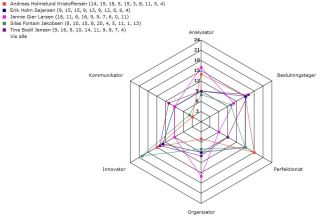
\includegraphics[width=0.5\textwidth]{itsaTRAP}
\caption{Figur, der viser resultatet af TRAP-testen.}
\label{trap}
\end{figure}

\subsubsection{Aftaler og koordinering}
Møder med kollegiekontoret er umiddelbart aftalt i et fåtal, og vi forventer ikke at kunne bruge tid fast til at udvikle sammen med dem “ved siden af”. Møder aftales med Lene Billeskov Jensen.

\subsection{Metode}

\subsubsection{Plan}
\begin{figure}[h!]
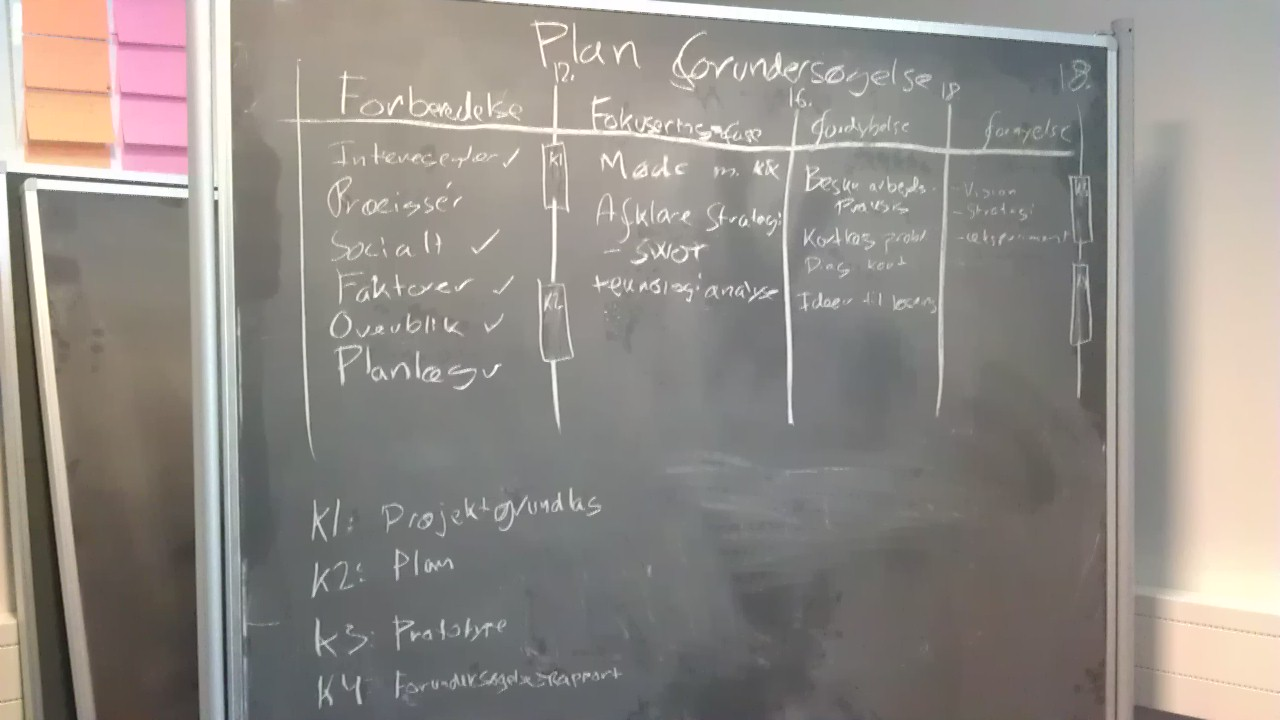
\includegraphics[width=0.5\textwidth]{forundersoegelsesplan.jpg}
\caption{Billede af planen.}
\end{figure}

\subsubsection{Teknikker og beskrivelsesværktøjer}
Til planen er allerede anvendt referencelinie-planlægning, og vi forventer at benytte os af interview/observation i forbindelse med at kortlægge arbejdspraksis (virksomhedsbesøg). Vi laver også en SWOT analyse, samt analyserer mål og strategi for at danne os et overblik og kortlægge problemstillingerne.

\subsubsection{Arbejdsform}
Internt i projektgruppen forventer vi at arbejde samme i løse grupper og individuelt i forbindelse med opgaveløsning. Samarbejdet med kollegiekontoret/styregruppe løftes med møder og email.
I det daglige vil vi bruge opslagstavler og alm. tavler til at holde styr på organiseringen.

\section{Fokusering}
\subsection{Virksomhedsbeskrivelse}
Hvis man er ung og skal i uddannelse eller er i gang med en uddannelse i Aarhus vil man med høj sandsynlighed benytte Ungdomsbolig Aarhus for at finde en bolig. På Ungdomsbolig Aarhus hjemmeside søger unge efter en ungdomsbolig. Hjemmesiden holder styr på unge der ansøger og boligforeninger som har boliger der skal beboes. De står for at udsende tilbud når boliger bliver frie, og for opsigelse af boliger.

  \subsubsection{Interne forhold}
De ansatte ved kollegiekontoret er primært kontorarbejdere der administrerer ungdomsboligerne igennem webbolig, der er et ERP værktøj for boliger. Arbejdet består bl.a i at tildele tilbud til ansøgere ved ledige boliger og opsige aftaler, samt rydde op i information som brugerne indtaster forkert, fx dobbelte ansøgninger. Opgaven er til dels papirtung da der anvendes udkørsler fra systemet som en oversigt over ledige boliger der skal tildeles. Arbejdsfordelingen er ret afklaret, og webbolig fungerer rimelig effektivt til at klare opgaven. Arbejdsgangen er tilrettelagt for at undgå fejl der kan medføre lejetab for de kollegier der administreres, omend i en idéel verden udføres der et arbejde der fra et teknisk synspunkt godt kunne automatiseres.

Ønsket om forandring ligger derimod i præsentationen af data ind/ud fra brugerne, der groft sagt er meget basal og uoverskuelig for mange. Der er ønsker om at gøre det lettere at udvælge relevante boliger i forbindelse med oprettelse af ansøgning, så det mindsker antallet af fejl brugerne laver, samt reducerer behovet for henvendelser fra ansøgere der ikke har kunnet overskue systemet.

  \subsubsection{Omgivelser}
Da man som ung boligsøgende under uddannelse reelt ikke har et andet alternativ end ungdomsbolig Århus har de tilnærmelsesvis opnået et markedsmonopol. Markedssituationen i sig selv må ses som værende stabilt, om end der typisk er større efterspørgsel end udbud. Det er dog ikke faktorer, som Kollegiekontoret som sådan hverken kan eller skal ændre på. Det er naturligvis nødvendigt at indrette sig efter den gældende lovgivning på området, og til dels også boligforeningerne, som de har et tæt samarbejde med.

\subsubsection{SWOT-analyse}
\begin{tabular}{ | l | r | }
\hline
Styrker & Svagheder \\ \hline
Markedsmonopol & Ingen konkurrence -> Ingen fornyelse \\
Stabilt marked & Umiddelbart ingen mulighed for markedsekspansion \\ \hline
Muligheder & Trusler \\
Teknologisk udvikling & \\
\hline
\end{tabular}
\newline
Idet Kollegiekontoret på dette område tilnærmelsesvis har monopol på markedet, har de ikke behov for at forny sig. De har dog heller ikke umiddelbart mulighed for det da markedets situation hele tiden er mere eller mindre stabil i forhold til målgruppen. De ønsker alligevel at levere en god service til deres brugere, hvor det ses at man kan udnytte den teknologiske udvikling til eks. at lave en bedre hjemmeside. Umiddelbart har de ingen eksterne trusler idet markedet er statisk.

  \subsubsection{IT-strategi}
Kollegiekontoret har ikke en decideret IT-strategi, men der er fokus på IT i deres aktivitetsmål. De relevante delmål går ud på at få bedre IT-systemer og lettere (kortere) arbejdsgange i administrationen. Disse mål skal opnås ved en mere sammenhængende elektronisk håndtering. Under mødet d. 16. april 2012 kom det også frem at de ønsker fremtidig fokus på brugervenlighed, som undgomsboligaarhus.dk skal afspejle. I den forbindelse har vi fået en behovspecifikation, som er baseret på feedback de har fået fra brugere.

  \subsection{Projektets arbejdsområder}
- Mere brugervenlig og tidssvarende brugeroplevelse af ungdomsboligaarhus.dk \newline
- Mere stabilt \newline
- Øget funktionalitet i præsentation af data og søgekriterier \newline

\section{Fordybelse}
\subsubsection{Referat af observationer og interviews}
\paragraph{Møde hos Kollegiekontoret d. 16/4-2012}
På mødet var der fokus på Kollegiekontorets bevæggrunde for ønske af et nyt system, og hvad de forventer det nye system skal kunne i forhold til det gamle. Der blev talt en del om at brugeren på den nye hjemmeside skal have en bedre oplevelse end på den gamle, samt at den nuværende hjemmeside har problemer med stabilitet, som den nye skal løse. Problemer med den nuværende arbejdssituation er udspecificerede i det diagnostiske kort nedenunder.
Desuden observerede vi, hvordan de bruger deres system i praksis og hvordan deres arbejdsproces med ansøgningerne og opdatering af hjemmesiden foregår. Dette havde til formål at finde frem til måder hvorpå det nye system kan effektivisere processen.

\subsubsection{Arbejdsgange}
\paragraph{Tildeling af bolig} foregår i webbolig, hvor en udlejningsmedarbejder har udkørsler med ledige boliger, der sammenholdes med en liste produceret i webbolig over ansøgere med længst anciennitet og evt. andre boligtilbud udsendt for nylig.

\paragraph{Retning af brugerdata} administreres ofte af medarbejderen, der må sidde med udkørsler og sammenligne brugere med enslydende navne for at rydde op i dobbelte ansøgere.

\subsection{Rige billeder}
Se Figur ~\ref{r_billede}
\begin{figure}
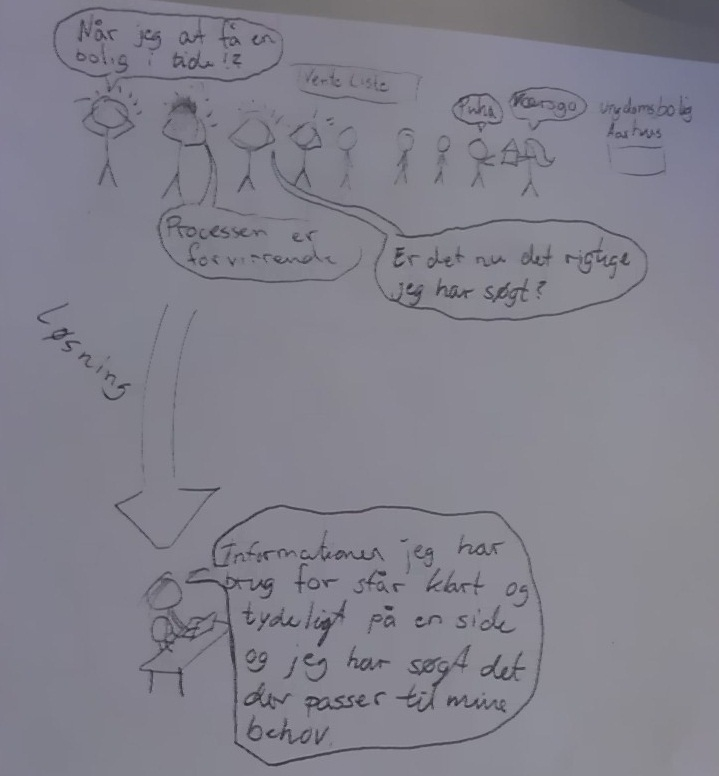
\includegraphics[width=0.5\textwidth]{rigtbillede}
\caption{Rigt billede.}
\label{r_billede}
\end{figure}

\subsection{Diagnostiske kort}
Se: Tabel ~\ref{d_kort}
\begin{table}
\caption{Diagnostiske kort}
\label{d_kort}
\begin{tabular}{| p{4cm} | p{4cm} | p{4cm} | p{4cm} |}
\hline
Problem & Årsag & Konsekvens & Ideer til løsning \\ \hline
Information forsvinder i systemet. \newline Siden kan kun bruges optimalt i IE. & Brugere logges ud under ansøgning. \newline Informationer kan forsvinde ved for mange opdateringer. \newline Bøvlet opdateringsproces. \newline Dårlig kode. & Frustrede ansøgere. \newline Klager. & Fejl lokaliseres. \newline Der startes forfra. \\ \hline

Siden er svær at navigere. & Layoutet er ikke intuitivt eller sammenhængende. & Brugeren finder ikke den ønskede information. & Mere gennemtænkt og brugervenligt layout. \\ \hline

Oprydning i information brugeren taster forkert. & Besværligt loginsystem & Ekstra arbejde med at vedligeholde data & Login systemet gentænkes \\ \hline

Bruger meget papir på store udkørsler. & Mange data der skal sammenholdes. & Papirspild & Bedre repræsentation af data i systemet \newline Opgraderet arbejdsplads med to skærme i stedet for én \\ \hline

Siden er uoverskuelig. & Mangel på søgekriterier. & Frustrerede ansøgere. \newline Ansøgere havner måske et sted de ikke havde tænkt sig. & Etablering af søgefunktion. \\ \hline

Besværlig login proces. & Autogenererede login oplysninger. & Ansøgerne opretter nye ansøgninger istedet for at bruge den allerede oprettede. & Brugerne får selv mulighed for at oprette et personligt login. \\ \hline

Nedbrud i systemer. & Forskellige leverandører af systemer til hjemmesider og webbolig. & Dyr vedligeholdelse og fejlretning. & Bedre kvalitet i løsninger. \newline Brug samme leverandør, giv dem et samlet ansvar. \\ \hline

\end{tabular}
\end{table}

\subsection{Mål}
\begin{enumerate}
\item Bedre browser kompatibilitet
\item Søgbare boliger med kriterier/valg
\item Nemt at ændre/vedligeholde informationer for personalet
\item Stabil hjemmeside
\item Brugervenligt layout
\item Individualiseret brugeroplevelse
\item Nemt login system
\item Integrering af geografisk placering i forhold til eks. uddannelsesinstitutioner
\item Integreres med webbolig
\end{enumerate}


\section{Fornyelse}
Samlet set er problemerne for Kollegiekontoret ikke så omfattende, og kræver ikke en større reorganisering af arbejdsgange, men hovedfornyelsen ligger hos kunderne som får en bedre service, lettere adgang til information og alt i alt en bedre oplevelse.

\subsection{Visioner om den samlede forandring}
\subsubsection{Vision 1}
Tilretning af eksisterende hjemmeside, hvor den oprindelige kode opgraderes med yderligere funktionalitet og nuværende fejl rettes så brugerne får en bedre oplevelse med hjemmesiden og der bliver færre inputfejl at rette i de bagvedliggende data.

Dennes vision er ikke let at implementere i praksis, da vi ikke har adgang til det eksisterende system internt, og da det er så ukompatibelt med de nye tanker om hvordan systemet skal virke at det ville være urentabelt at bruge denne fremgangsmåde. Fordelen kunne være at det ville være en billig lappeløsning på problemerne, men de eksisterende småproblemer kan vokse sig større. Det kunne også være at systemet er konstrueret dårligt og derfor ville tage lang tid at sætte sig ind i systemet og rette på det uden at forårsage nye fejl.

\subsubsection{Vision 2}
Gentænkning af systemet og efterfølgende ny implementation, hvor der skrives helt ny kode helt fra bunden af, og alle eksisterende fejl derfor elimineres og ny funktionalitet kan tilføjes uden hensyntagen til kompatibilitet med oprindelige systemer.

Dette kan gennemføres i praksis og være en rentabel løsning. Det tager sandsynligvis ikke længere tid end at rette i den eksisterende løsning, og resultatet vil være mere helt, og lettere og billigere at opdatere i fremtiden, og det vil være lettere at udføre vision 3.

\subsubsection{Vision 3}
Implementation af integrering af Webbolig, som er en udbygning af scenariet beskrevet i Vision 2, og indebærer fuld kompatibilitet med systemet Webbolig.

En fuld integration vil være meget svær at kunne lave på den afsatte tid. Det er derfor ikke noget vi vil bestræbe os på at opnå, men det er et oplagt fremtidsprojekt.

\subsection{Strategi og plan for realisering}
Taget i betragtning af den stramme tidsplan og manglende kendskab til eksisterende løsning, er vision 2 en realistisk løsning for skoleopgaven, men vision (2+)3 er den endelige løsning for Kollegiekontoret. Det eksisterende system er en meget forældet platform der kan blive meget dyr at vedligeholde i fremtiden efterhånden som færre udviklere har kendskab til systemet.

\subsection{Mock-ups}
Se bilag

\section{Konklusion på forundersøgelse}
Vi har været godt rundt om Kollegiekontoret, og afklaret at de har et reelt behov for en tidsvarende hjemmeside der giver en bedre servicering af ansøgere. Der er lagt op til at projektgruppen, som omfatter os som studerende implementerer vision 2 bl.a. pga. den begrænsede tid. Den manglende integrering med webbolig får ikke konsekvenser for Kollegiekontoret da de ikke regner med at få et kørende system.

%Please edit below this point by editing files on the git repo! - AS IF
% Lolediting trollolololol
%FFFFFFFUUUUUUUUUUUU
%Seriøst..
%Det fungerer jo ikke i multiplayer.. latexforholdet er anstrengt nok i forvejen


%NYNYNYNYNYNYNY UDVIKLINGSPROJEKTSRAPPORT

\chapter{Udviklingsprojekt}

Eftersom vi under forundersøgelsen er kommet frem til at den mest rentable løsning vil være at implementere en ny webside fra bunden, kan udviklingsprojektet starte.

I rapporten herunder har vi dokumenteret hvordan processen er forløbet, samt redegjort for det produkt, som vi har lavet i sammenarbejde Kollegiekontoret.

\section{Projektetablering}

For at projektet skal have et solidt fundament med en god organisering, har vi valgt at analysere vores udgangspunkt så vi ved, hvor vores styrker ligger, og hvor der kan opstå forhindringer, som vi skal forsøge at styre udenom.

Fra starten har vi lavet teambuilding, fx ved at tage en øl sammen og lave aftaler om organisering og skabe entusiasme for projektet. Vi har også haft en indledende snak med Kollegiekontoret om at arbejde med en agil metode, så vi kan have en tæt kontakt gennem hele forløbet.

\section{Projektets organisering}

Hele teamet har taget en TRAP-test (se ~\ref{trap}) for at vurdere vores personressourcer. Testen viste at holdet har balance i de fleste punkter men har en manglende evne i kommunikation. Holdet har ellers medlemmer, som har mindst 15 point i de andre kategorier mens den højeste scorer i kommunikation kun er ca. 11 point. Selvom kommunikationen er lav kender hele teamet hinanden forholdsvis godt, da vi har arbejdet sammen flere gange før.

TRAP-testen skal ikke ses som endegyldige fakta, men mere skal bruges som en test der giver et fingerpeg om hvordan gruppen er sammensat, og hvordan de enkeltes styrker dækker de andres svagheder ind. Testen giver også et overbliksbillede over gruppens generelle svagheder, som vi skal være særligt opmærksomme på. De områder hvor flere gruppemedlemmer er mindre stærke, kræver fælles indsats for at opnå bedst mulig synergi på området.

\subsection{Turboanalyse}

For at kunne forudse mulige problemområder og finde de områder hvor vi kan udnytte teamets stærke sider til fulde, har vi valgt at lave en TURBO-analyse.

\noindent

\begin{tabular}{| p{3cm} | p{3cm} | p{3cm} | p{5cm} |}

\hline

Mål og vilkår & Særlig styrke & Særlig svaghed & Mulige beslutninger \\ \hline

Teknikken &  & Usikkerhed om nuværende anvendt teknik & Vi kan starte fra bunden, fremfor at bygge ovenpå eksisterende \\ \hline

Udviklerne &  & Uerfarne & Vi skal være forberedte på at få hjælp fra undervisere. \\ \hline

Resultat & Skal ikke blive færdigt, da det ikke er målet &  & Fokuser på at lære noget \\ \hline

Brugerne & Brugerne har svært ved at fravælge produktet &  &  \\ \hline

Omgivelserne &  & Projektgruppen har andre opgaver under forløbet & Afstem forventninger og prioriteter \\ \hline

& \multicolumn{3}{| c |}{Projektets strategi} \\ \hline

Sammenfatning & \multicolumn{3}{| p {11cm} |}{ Vi starter umiddelbart udviklingsprojektet fra bar bund, og satser ikke på at levere et færdig produkt, men at vi lærer noget af proccessen ved et udviklingsprojekt. Vi vil også være eksperimenterende i idéerne så der kan komme noget brugbart og inspirerende ud af projektet for alle parter. } \\ \hline

\end{tabular}

\subsection{Risikoanalyse}

Herunder har vi forsøgt at opstille de risikofaktorer, som omstændighederne for projektet ligger under for. Risikofaktorerne omhandler interessenterne, omgivelserne og processen. På denne måde kan vi foregribe eventuelle problemer og forhåbentligt afværge dem. \newline
\vspace{1cm}
\noindent

\begin{tabular}{| p {5cm} | p{2cm} | p{2cm} | p{2cm} | p{4cm} |}

\hline

Risici & Sandsynlighed & Alvorlighed & Riskotal (Sandsynlighed * alvor) & Håndtering \\ \hline

For lidt viden om det eksisterende system & 37 & 3 & 111 & Kommunikere ofte med kunden \\ \hline

Miskommunikation med kunden & 10 & 7 & 70 & Opnå enighed i gruppen om kundens udmeldinger \\ \hline

Manglende kommunikation internt i projektteamet & 5 & 8 & 40 & Være åbne overfor hinanden \\ \hline

Manglende teknisk viden hos udviklerne & 25 & 3 & 75 & Søge hjælp ved lærere, hinanden og internettet \\ \hline

Sygdom i teamet & 75 & 3 & 225 & Tage højde for dette i planlægning og metodevalg \\ \hline

Tekniske problemer med udviklingsværktøjer & 80 & 1 & 80 & Vælge værktøjer vi ved fungerer godt og søge teknisk hjælp hvis det alligevel ikke fungerer \\ \hline

Mangelfuld planlægning fra udviklernes side & 10 & 4 & 40 & Holde møder ofte og vælge en udviklingsmetode der understøtter tæt kommunikation \\ \hline

Problemer med skolens net & 100 & 9 & 900 & Tage et andet sted hen for at arbejde \\ \hline

\end{tabular}

\subsection{Metodevalg}

Projektets karakter gør det oplagt at bruge agile metoder, da der er brug for en tæt kontakt mellem os som udviklere og Kollegiekontoret, da der er en vis usikkerhed i kravene til systemet og ikke så klare retningslinjer for dets funktionalitet. Personalet er ikke særligt teknisk anlagt, og vi har ikke noget stort indblik i det eksisterende systems implementation og funktioner.

\begin{figure}

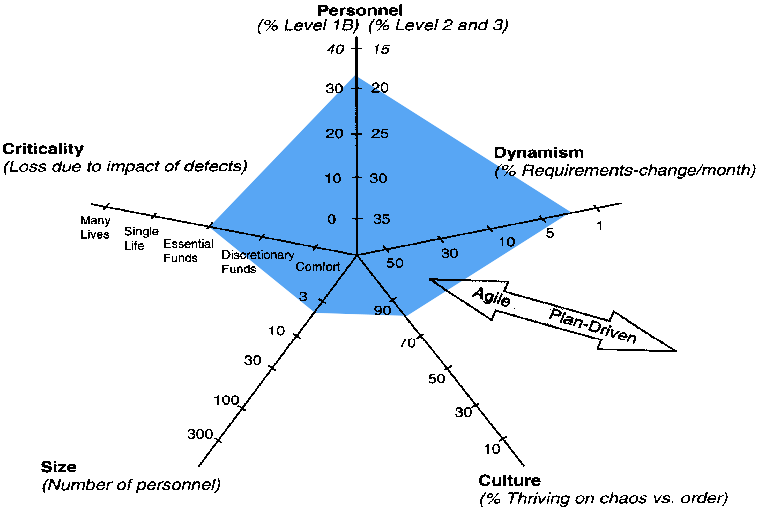
\includegraphics[width=0.5\textwidth]{amoebe}

\caption{Boehms Dimensioner}

\label{amoeb}

\end{figure}

Figur ~\ref{amoeb} viser forholdet mellem opgavens kompleksitet, antallet af personer på projektteamet, kundens afhængighed af systemet, projektmedlemmernes evne til at arbejde agilt og produktkravenes foranderlighed.

Foranderlighed, agil arbejdsevne og afhængighed af systemet er faktorer der peger på at vælge en plandreven metode, men agil arbejdsevne er dels vurderet så højt fordi vi aldrig har arbejdet med det før, og den erfaring kan kun komme ved at prøve og få erfaringer.

Derfor har vi valgt at vi gerne vil arbejde med en agil metode, der bl.a. sikrer at vi når at lære noget om udviklingsprocessen involveret i det, og fordi det også har være salgstalen overfor Kollegiekontoret, så de får en smag for den side af udviklingsverdenen inden de endeligt får løst deres behov for en ny hjemmeside.

Vi har endeligt valgt SCRUM som udviklingsmetode, da vi gerne selv vil prøve at arbejde efter en ny metode, og da principperne i SCRUM passer godt til projektets lidt usikre og udefinerede karakter. Vi krydrer vores SCRUM med nogle af elementerne fra XP som vi mener kan gavne vores udviklingsprojekt.

Pair programming mener vi er en god praktik da det er første gang vi skal udvikle en opgave af større omfang i et nyt udviklingssprog, er det en god måde at opveje for hinandens usikkerhed.

Informative workspace opsætter vi for at have informationer samlet og tilgængelige. Ligeledes er det vigtigt at alle har koden tilgængeligt til at arbejde på, og vi vil lægge energi i at have versionsstyring til koden.

Sit together er en god udviklingspraksis, fordi der er flere øjne over koden på en gang, og fordelen i form af synergieffekt ved at forene evner og overblik opvejer det kaotiske ved at arbejde flere mennesker på den samme opgave. Dette hjælper med at spotte problemer når de opstår, hurtigere end hvis man kodede selv.

Overordnet set er vi alle ansvarlige for at projektet går godt, da en af hovedkarakteristika ved agil udvikling er en flad organisatorisk struktur med fælles ansvarsfordeling i et projektteam. Teamet har en ansvarlig for overholdelse af metoden, en SCRUM-master. Der er i metoden også brug for en ansvarlig til at opretholde en Product Backlog for kunden, denne er Product Owner.

\subsection{Fordeling af roller}

SCRUM-Master: Tina Jensen \newline

Product Owner: Jannie Gier Larsen \newline

Dokument- og versionsstyring: Andreas Kristoffersen \newline


\section{Projektplanlægning}

\subsection{Product backlog}

På baggrund af møde med Kollegiekontoret under forundersøgelsen, udarbejdede teamet en product backlog med en komplet liste over deres og slutbrugeres ønsker for systemet. Der blev senere holdt et møde, hvor repræsentanter fra Kollegiekontoret godkendte features listen uden ønske om ændringer af denne. Herunder kan det ses, hvad vi kom frem til.

\subsubsection{Features}

\begin{enumerate}

\item Der skal kunne vælges mellem en dansk- og engelsksproget version af siden. Estimeres til 3 units.

\item Man skal kunne se en oversigt over de fremsøgte boliger med sammenlignelig info om hver bolig. Estimeres til 8 units.

\item Understøttelse af de mest udbredte browsere, herunder de nyeste to versioner af Mozilla, Safari, Opera og IE, samt de tre nyeste versioner af Chrome. Estimeres til 17 units.

\item Nyheder vises på forsiden Estimeres til 2 units.

\item Content management system, hvor webmasteren skal kunne rette nyheder, boliger og tekst generelt. Estimeres til 80 units.

\item Finde boliger ved at bruge avanceret søgning. Ting man f.eks. kan søge på: m$^{2}$, husdyr, børn, eget bad og køkken, antal værelse og hvilken internet og tv udbyder man vil have. Estimeres til 20 units.

\item Bolig kvik-søgning på forsiden. Man skal kunne søge på antal personer (1 eller 2) og postnr. Estimeres til 5 units.

\item En liste med boliger der har ingen eller kort ventetid til studerende i akut bolignød. Estimeres til 2 units.

\item Man skal kunne sortere de fremsøgte boliger efter pris, ventetid, beliggenhed. Beliggenhed er umuligt at estimere på nuværende tidpunkt. Range 2-100.

\item Hjemmesiden skal være brugervenlig så man hurtigt kan finde en bolig der passer til ens behov. Information skal derfor være nemt tilgængeligt og struktureret. Estimeres til 17 units.

\item Mulighed for brugerne at logge ind med emails istedet for bruger nummer. Er udgangspunkt og estimeres derfor til 1 unit.

\item Boliger skal placeres med geografisk lokation på et kort

\item Integration med webbolig, så informationsmedarbejderne nemt kan bearbejde ansøgningerne.

\end{enumerate}

\subsection{Release planning meeting}

Vi valgte at estimere vha. planning poker. 11. punkt, der vedrører login via. email estimeres til 1 unit. De øvrige features estimerede vi  ud fra denne feature og prioriterede dem derefter udfra bubblesort metoden. Resultatet er vist ovenover.

Foruden at hjælpe os til at estimere, gav planning poker også anledning til at diskutere de enkelte user stories, og hvad de hver især indebærer. Da vi ved en user story kom frem til et spænd på 2-100, fandt vi ud af at der ikke var taget højde for nødvendigheden af et Content management system. Som det ses ud fra listen over features, har vi estimeret det til at være meget tidskrævende at implementere i forhold til mange af de andre features.

Vi er kommet frem til følgende done kriterie, som passer til den valgte udviklingsmetode: Code complete, merged og gennemført peer review..

For at fastsætte, hvor lang tid en unit udgør, implementerede vi user story 11. Vi kom frem til at én unit svarer til ca. 70 minutters pair programming.

Da vi havde estimeret os frem til en idé om, hvor lang tid det vil tage at implementere systemet, fastsatte vi første og eneste release til d. 21 maj 2012. Pga. den korte tidsperiode, vurderede vi at vi ikke kan nå at implementere alle features inden deadline.

Vi har valgt medtage festures 1-11 i release, da features 12 og 13 er for omfattende. De kræver dels at vi får adgang til Kollegiekontorets bagvedlæggende system, og dels at det kan koste penge at integrere systemet med kort. Begge features vurderes desuden til at være meget tidskrævende, idet udviklerne skal være fortrolige med API’erne.

\subsection{Releaseplan}
På figur ~\ref{release_plan} ses vores releaseplan.
\begin{figure}
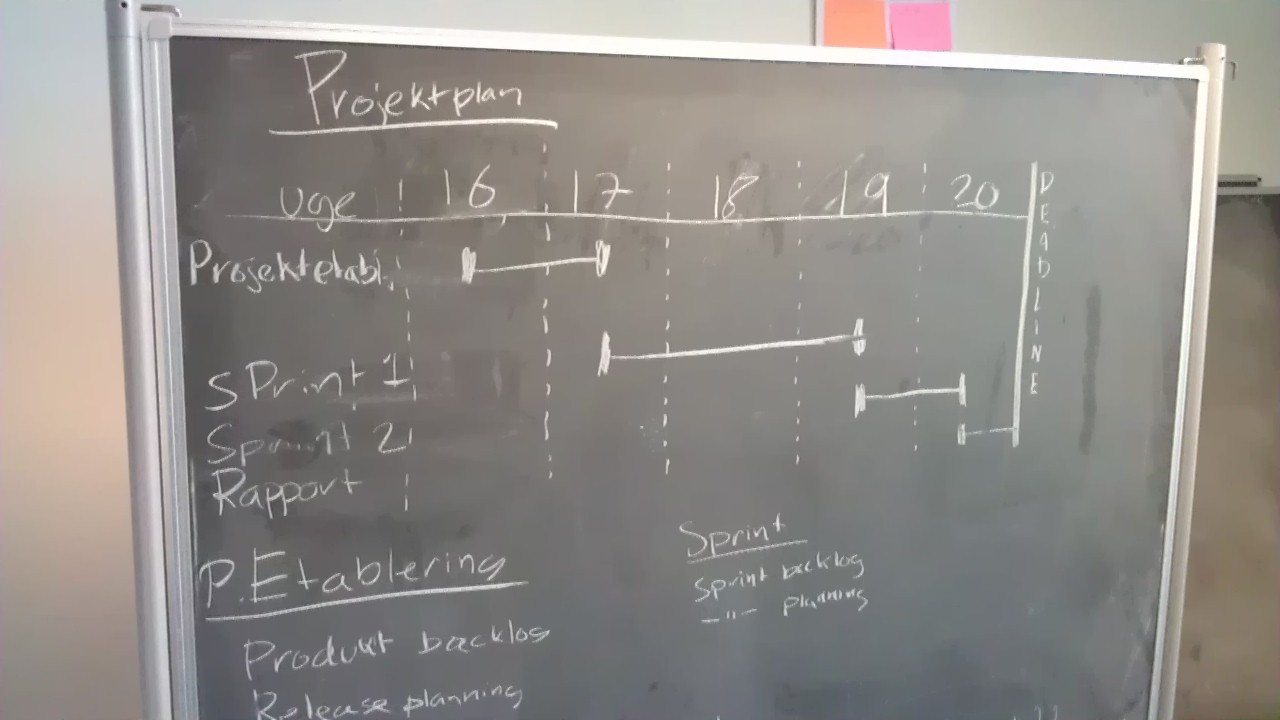
\includegraphics[width=0.5\textwidth]{releaseplan}
\caption{Releaseplan}
\label{release_plan}
\end{figure}

\section{Iterationer}

Herunder har vi dokumenteret, hvordan vi konkret har valgt at bruge SCRUM og XP i det daglige.

Stedet vi havde valgt at have vores ‘base’ var i vores klasselokale. Rundt om bordet hvor vi sad havde vi stillet tavler op som vi kunne skrive på og hænge vores plancher op som f.eks. burn-down charts og scrumboards. Af mangel på bedre muligheder, fungerede tavlerne også som rumopdelere, så gruppen sad i en såkaldt “cubicle”.

\begin{figure}
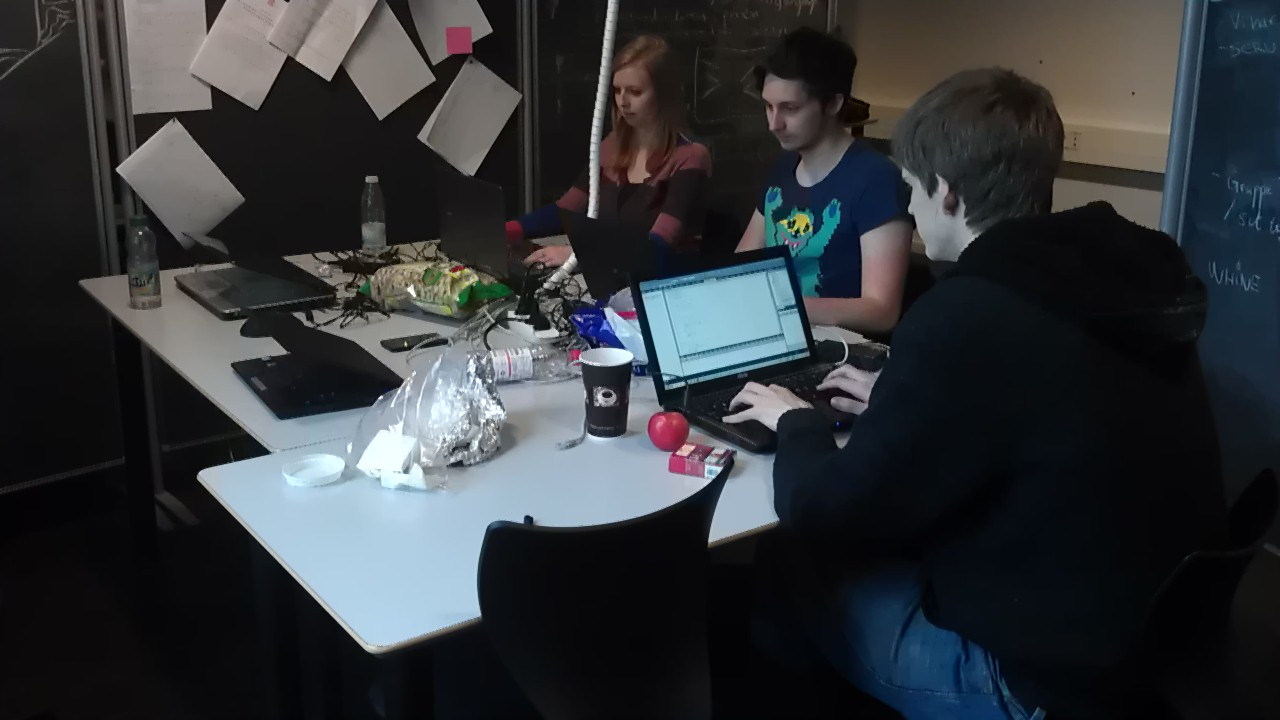
\includegraphics[width=0.5\textwidth]{ziriuzarbejde}
\caption{Vores cubicle}
\label{cubicle}
\end{figure}

Som tidligere nævnt har vi benyttet os af planning poker til at estimere vores user stories og tasks. Det har gjort, at vi nemt har kunnet planlægge vores sprints, hvilket har været meget rart.

User stories og tasks blev arrangeret på et traditionelt scrumboard (Fig. ~\ref{s_board}), hvor tasks kan være hhv. “not checked out”, “checked out”, og “done” (som er de tasks, der opfylder vores done kriterie).

Denne anvendelse har gjort vores user stories mere håndgribelige, og har betydet, at vi nemmere har kunnet følge med i hvor langt vi er kommet.

\begin{figure}
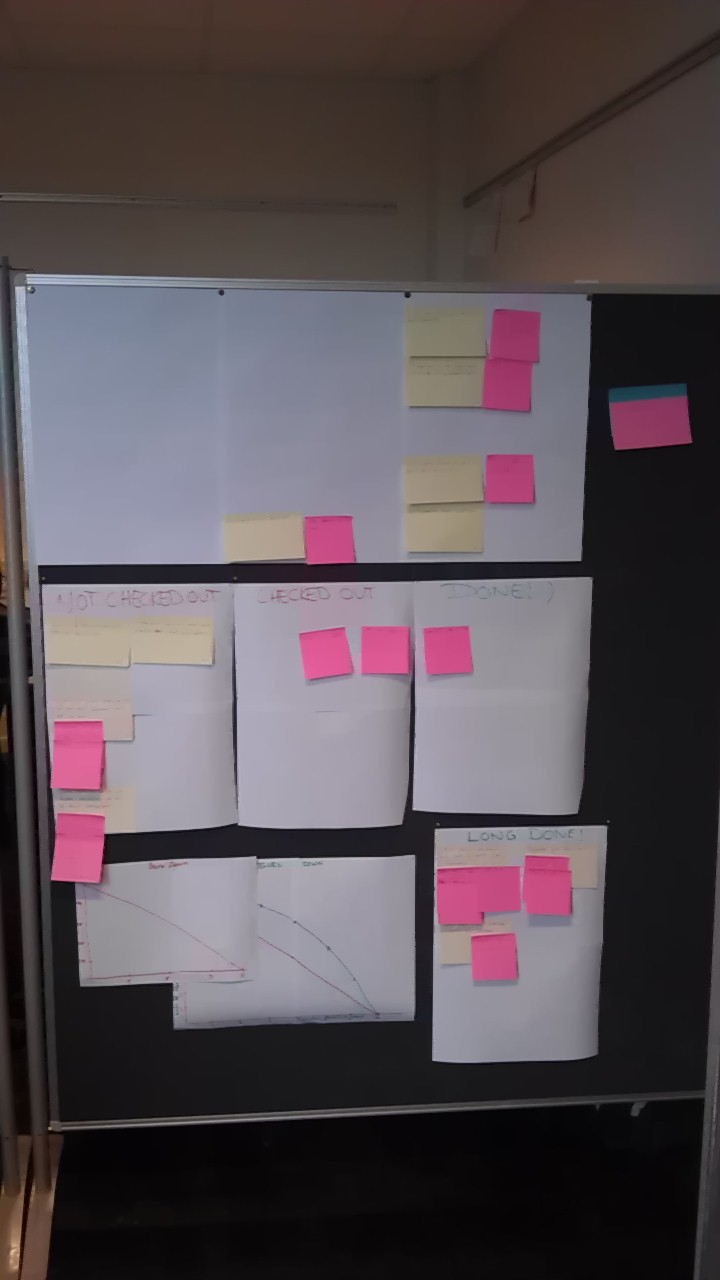
\includegraphics[width=0.5\textwidth]{scrumboard}
\caption{SCRUM board}
\label{s_board}
\end{figure}

Til at styre den daglige planlægning, har vi holdt standup-meetings á 10 minutters varighed. De blev brugt til at belyse dagsordenen, blotlægge eventuelle forhindringer og snakke om sprintets generelle status.

Pair programming og sit together, fra XP, har også været praktikker, som har fungeret rigtig godt og resulteret i at vi alle er blevet stærkere i de benyttede udviklingsværktøjer.

Desuden har vi gennem hele projektet har vi benyttet os af slack, som er endnu en af XP’s praktikker, og det har medført at der har været en god koncentration om opgaven når vi har arbejdet aktivt på projektet. Slack har været i form af sociale aktiviteter i gruppen, som har holdt humør og energi oppe.

\subsection{1. sprint}

\subsubsection{Sprint planning meeting}

\begin{tabular}{| l | l |}

\hline
Sprint længde & 1\nicefrac{1}{2} uge \\ \hline
Arbejdsdage i dette sprint & 7 dage \\
\hline
\end{tabular}
\newline
\vspace{1cm}
\noindent
\begin{tabular}{| p{4cm} | p{4cm} | p{4cm} | p{4cm} |}
\hline
Team medlem & Total antal tilgængelige dage & Tilgængelige timer per dag & Total antal timer \\ \hline
Silas & 7 & 6 & 42 \\ \hline
Tina & 7 & 6 & 42 \\ \hline
Andreas & 7 & 6 & 42 \\ \hline
Jannie & 5 & 6 & 30 \\ \hline
Erik & 5 & 6 & 30 \\
\hline
\end{tabular}
\newline

Vi startede første sprint med at estimere vores velocity, som er fastsat til omkring 12 units per dag. Vi er kommet frem til at der er 186 timer tilgængelig til sprintet, og har vurderet at for at overhovedet at kunne løse story 5 på 80u skal den passe ind her. Da story 4 er en byggesten til story 5 og til sammenligning ubetydelig lille, ender sprint 1 på at omfatte 82u eller 95 pair programming timer. For at få det til at passe sammen kan al programmering dog ikke være i par.

Formålet med sprintet er at få fremstillet grundpillen for resten af systemet og få det op og køre, så der er noget at arbejde videre på.

\begin{figure}
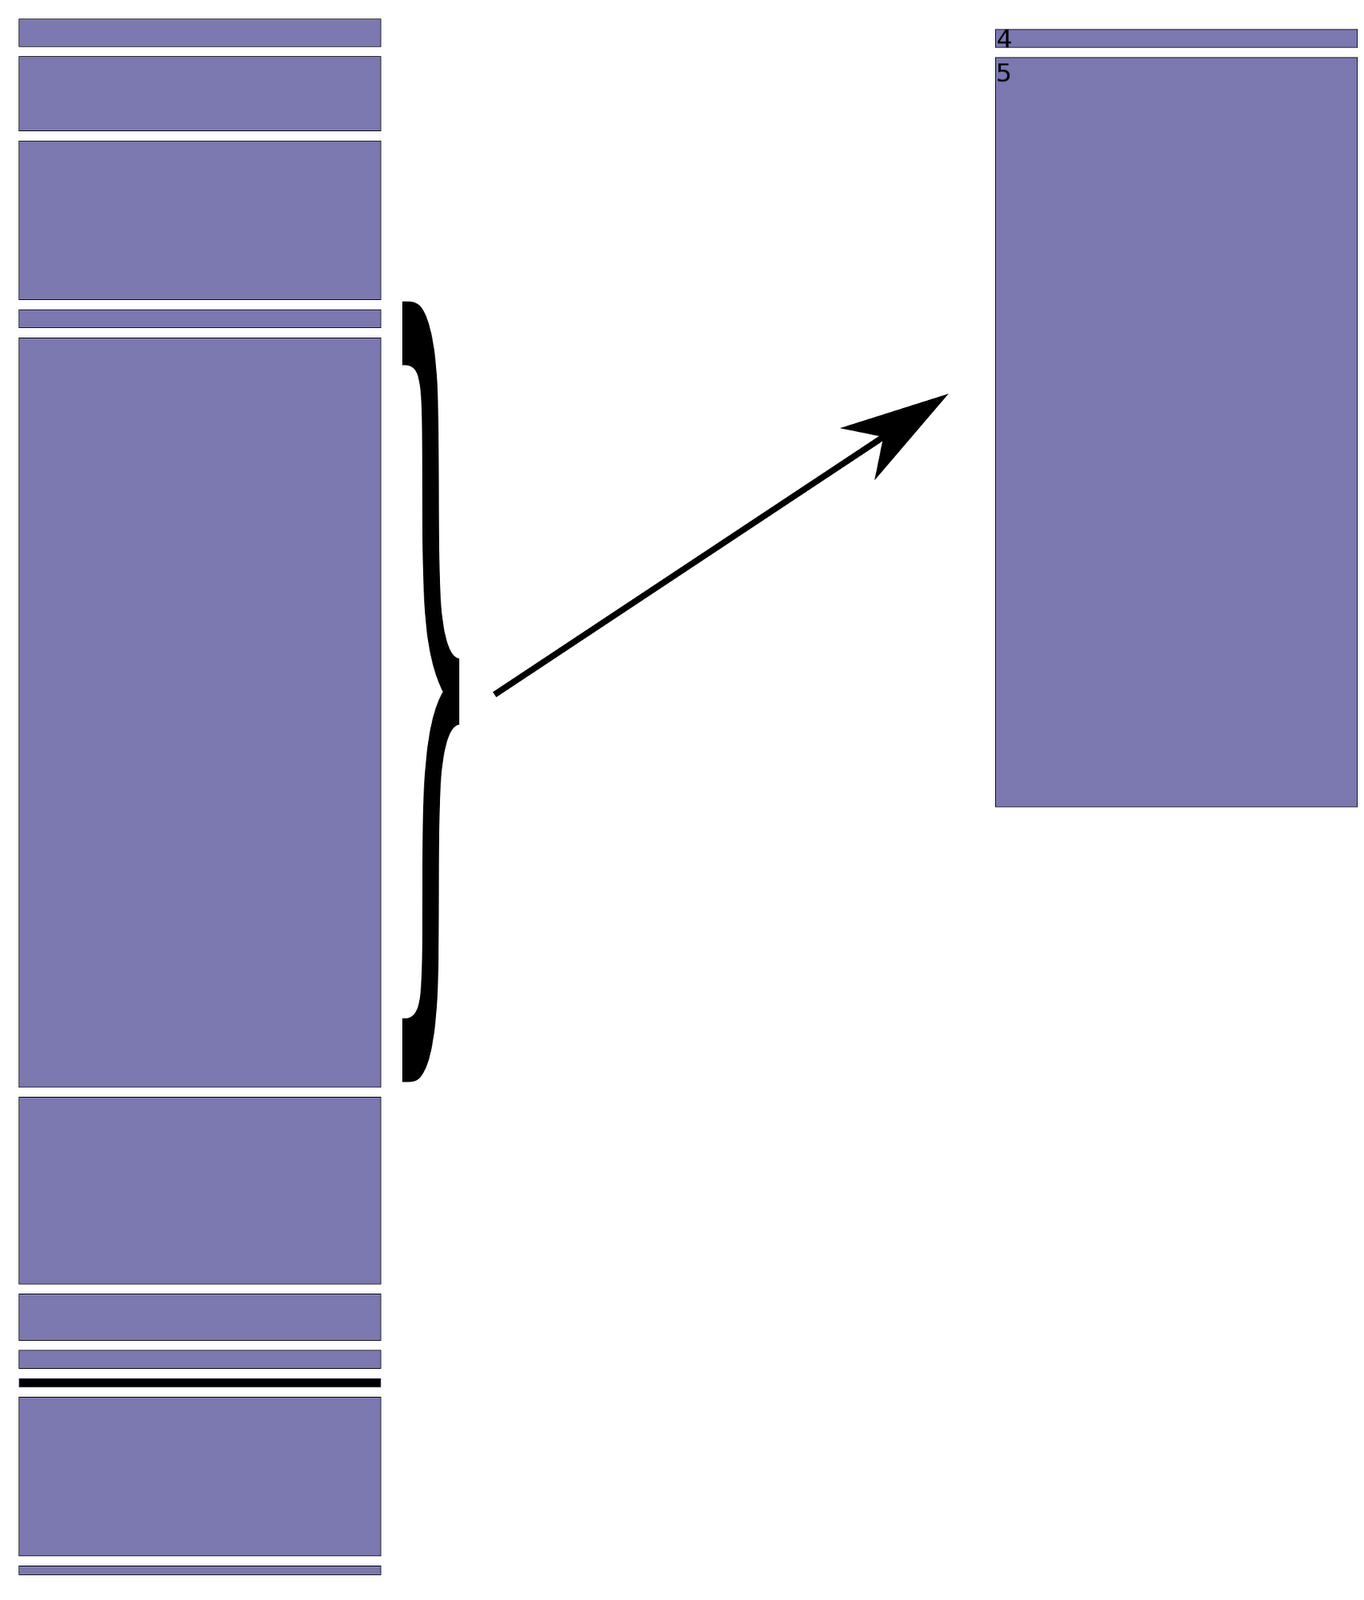
\includegraphics[width=0.5\textwidth]{sprint1log}
\caption{Grafisk fremstilling af sprint backlog}
\label{sprintlog1}
\end{figure}

\subsubsection{Sprint review}

Sidste dag i sprintet blev der lagt en prøve version af sitet på nettet og derefter tog vi ind til Kollegiekontoret for at lave et sprint review og derved vise dem, hvad vi har nået i sprintet. Lene var hovedsageligt positiv overfor den nuværende implementation og syntes, at vi har ramt godt i forhold til deres ønsker, samt at systemet ser intuitivt ud at bruge. Vi snakkede dog om, hvorvidt man kan fokusere for meget på brugervenlighed. Det blev derfor aftalt, at der skal oprettes en bruger med admin-rettigheder, så flere brugere hos Kollegiekontoret kan prøve systemet på egen hånd på et aftalt tidspunkt, og vurdere om der skal laves ændringer. Desuden blev det aftalt at vi skulle fortsætte med implementationen i samme stil som hidtil.

\subsubsection{Sprint retrospective}

Efter mødet satte teamet sig ned og snakkede om hvordan sprintet var forløbet. Det foregik ved at bruge en tavle med to spalter, hhv. “what works” og “what could be improved”. På den positive side fandt vi ud af, at vi havde nået vores mål, at scrum board og backlogs samt gruppe programmering/sit together fungerede godt. Jf. burn down chartet havde sprintet en hård start, hvilket kan skyldes nye arbejdsmetoder samt generelle opstartsproblemer, men efter tilvænningsperioden blev gruppen mere effektiv. Det at bruge scrum værktøjer som boards og backlogs gjorde det meget nemmere at koordinere arbejdet og det gav en positiv følelse at kunne følge sprintets fremskridt hele tiden. Modsat fandt vi ud af, at vi ikke har været gode til at holde standup meetings. Det vil vi førsøge at forbedre i næste sprint. Desuden kunne vi ikke undgå at komme ind på at omgivelserne ikke er optimale, og at problemer med skolens internet har været en stor hindring for vores arbejde.

\subsection{2. sprint}
\subsubsection{Sprint planning meeting}

\begin{tabular}{| l | l |}

\hline
Sprint længde & 1 uge \\ \hline
Arbejdsdage i dette sprint & 4 dage \\
\hline
\end{tabular}
\newline
\vspace{1cm}
\noindent
\begin{tabular}{| p{4cm} | p{4cm} | p{4cm} | p{4cm} |}
\hline
Team medlem & Total antal tilgængelige dage & Tilgængelige timer per dag & Total antal timer \\ \hline
Silas & 4 & 6 & 24 \\ \hline
Tina & 4 & 6 & 24 \\ \hline
Andreas & 4 & 6 & 24 \\ \hline
Jannie & 4 & 6 & 24 \\ \hline
Erik & 4 & 6 & 24 \\
\hline
\end{tabular}
\newline

Andet sprint startede igen ud med et sprint planning meeting. Vi fastsatte sprintets velocity til 48 units og udvalgte vha. den fastsatte estimering user stories svarende til dette ud fra prioriteringen. Da vi ikke kunne få det til at gå op med den fastsatte velocity, blev vi på baggrund af erfaring fra første sprint, enige om at tage en stor user story med (nr. 6 som er implementering af advanceret søgning), som går ud over vores velocity. Der er derfor risiko for at alle tasks for den pågældende user story ikke bliver færdig, hvor vi i så fald overdrager den/dem til næste sprint.

Formålet med dette sprint var hovedsageligt, at implementere user stories der vedrører slutbrugerne.

\begin{figure}
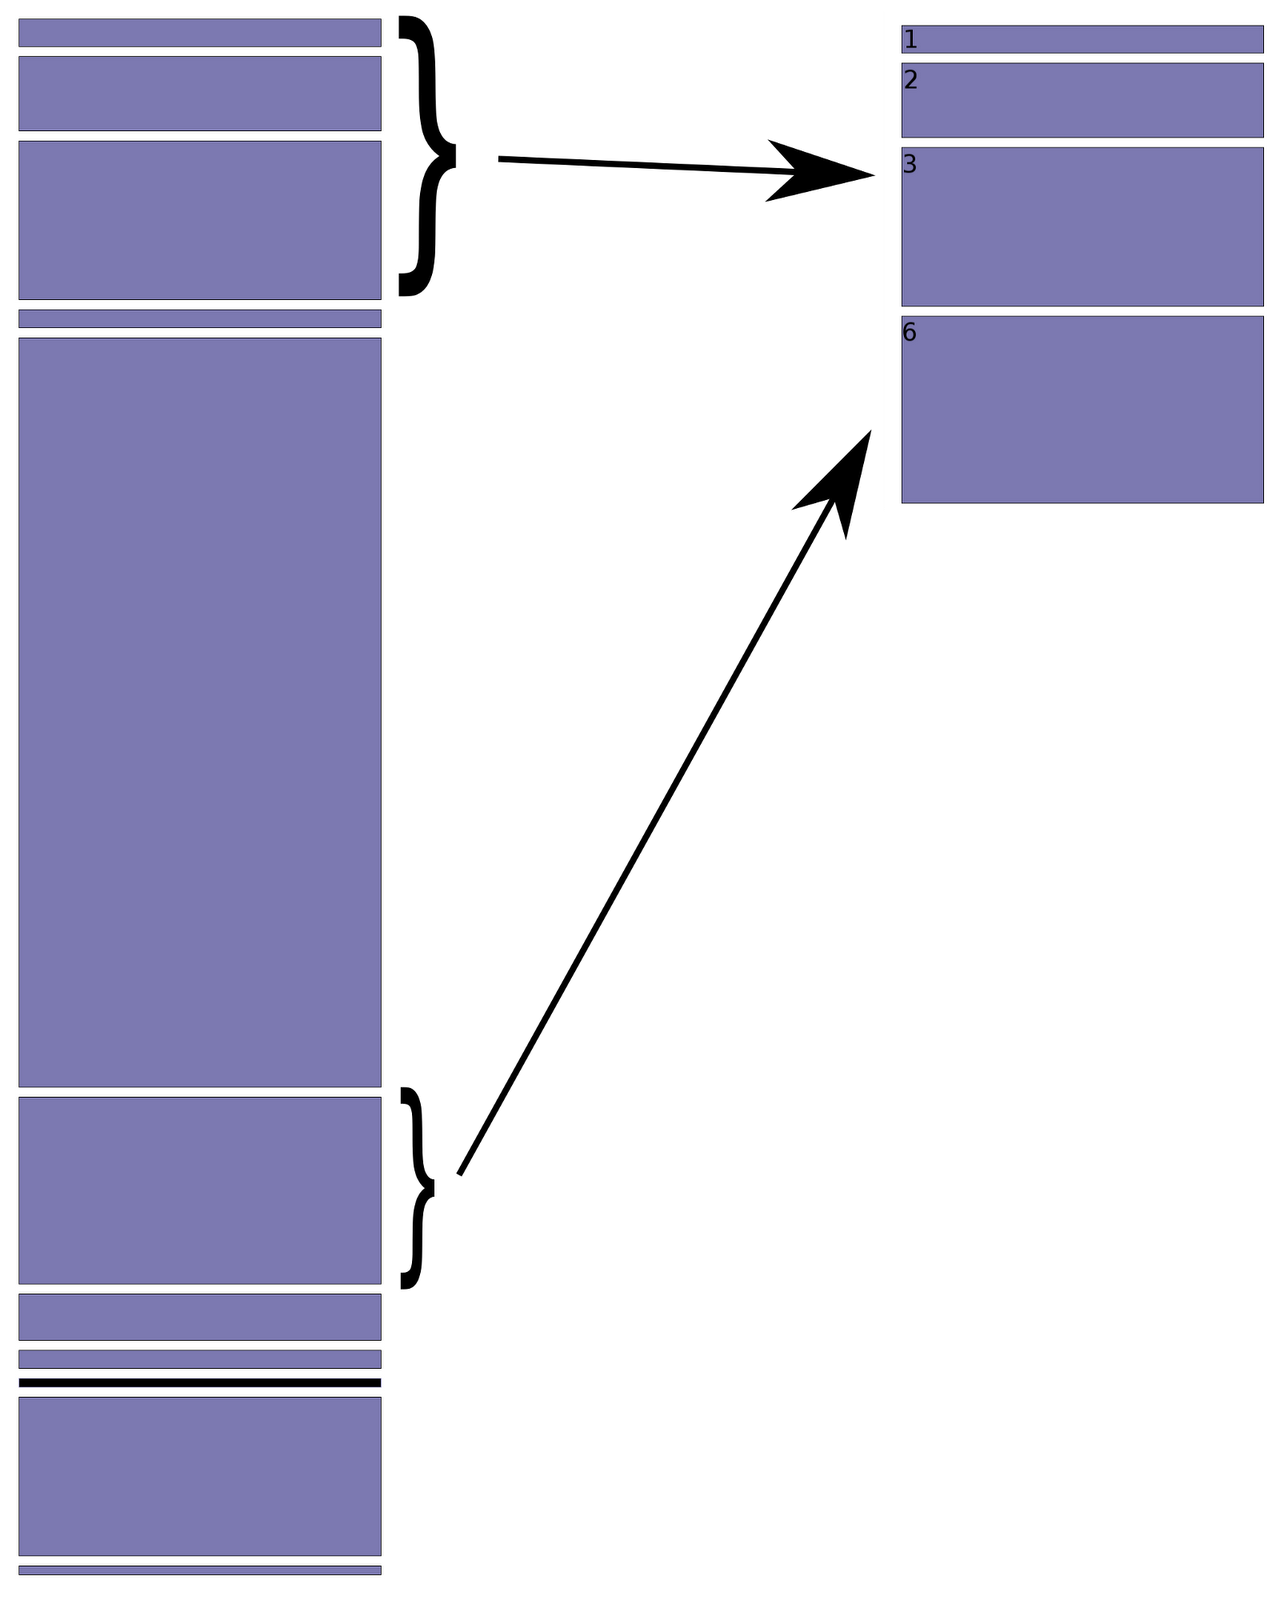
\includegraphics[width=0.5\textwidth]{sprint2log}
\caption{Grafisk fremstilling af sprint backlog}
\label{sprintlog2}
\end{figure}

\subsubsection{Revision af product backlog}

Under sprintet kom det pludselig frem, at en essentiel del af funktionaliteten ikke er dækket ind, nævnlig den del, der vedrører ansøgning af boliger. Under hidtidige møder med Kollegiekontoret er emnet ikke blevet bragt op. Det viser, at det er vigtigt at være påpasselig med at user stories dækker al funktionalitet og at ingenting er underforstået, men skal blotlægges og dokumenteres. På grund af vores valg af en agil udviklingsmetode er det nemt at tilføje funktionalitet til systemet - det handler blot om at tilpasse fremtidige releases og sprints herefter.

De nye user stories er beskrevet således:

\begin{enumerate}

\item Brugere skal kunne oprette en profil der indeholder generelle brugeroplysninger, samt oplysninger om hvornår de ønsker en bolig fra og tidsperioden de forventes under uddannelse.

\item Når en bruger er inde på en bolig’s side, skal det være muligt at oprette en boligansøgning baseret på dennes info og brugerens oplysninger.

\end{enumerate}

Idet første release lægger fast, er det ikke muligt at tilføje funktionaliteten herunder, så vi har valgt ikke at estimere disse user stories. Dog vurderer vi, at de trods deres vigtighed ikke er særlig omfattende, så hvis der var flere releases inden deadline ville det ikke kræve megen tid at implementere dem.

\section{Kvalitetsbeskrivelse}


\section{Projektevaluering}


\chapter{Produktet}
\section{Kravspecifikation}
%Indsæt billede backlog

\section{Testcases}
%lolwut

\section{Modeller}


\section{Design}


\section{Kode}
%Indsæt interessant kode

\chapter{Bilag}

\begin{SCfigure}
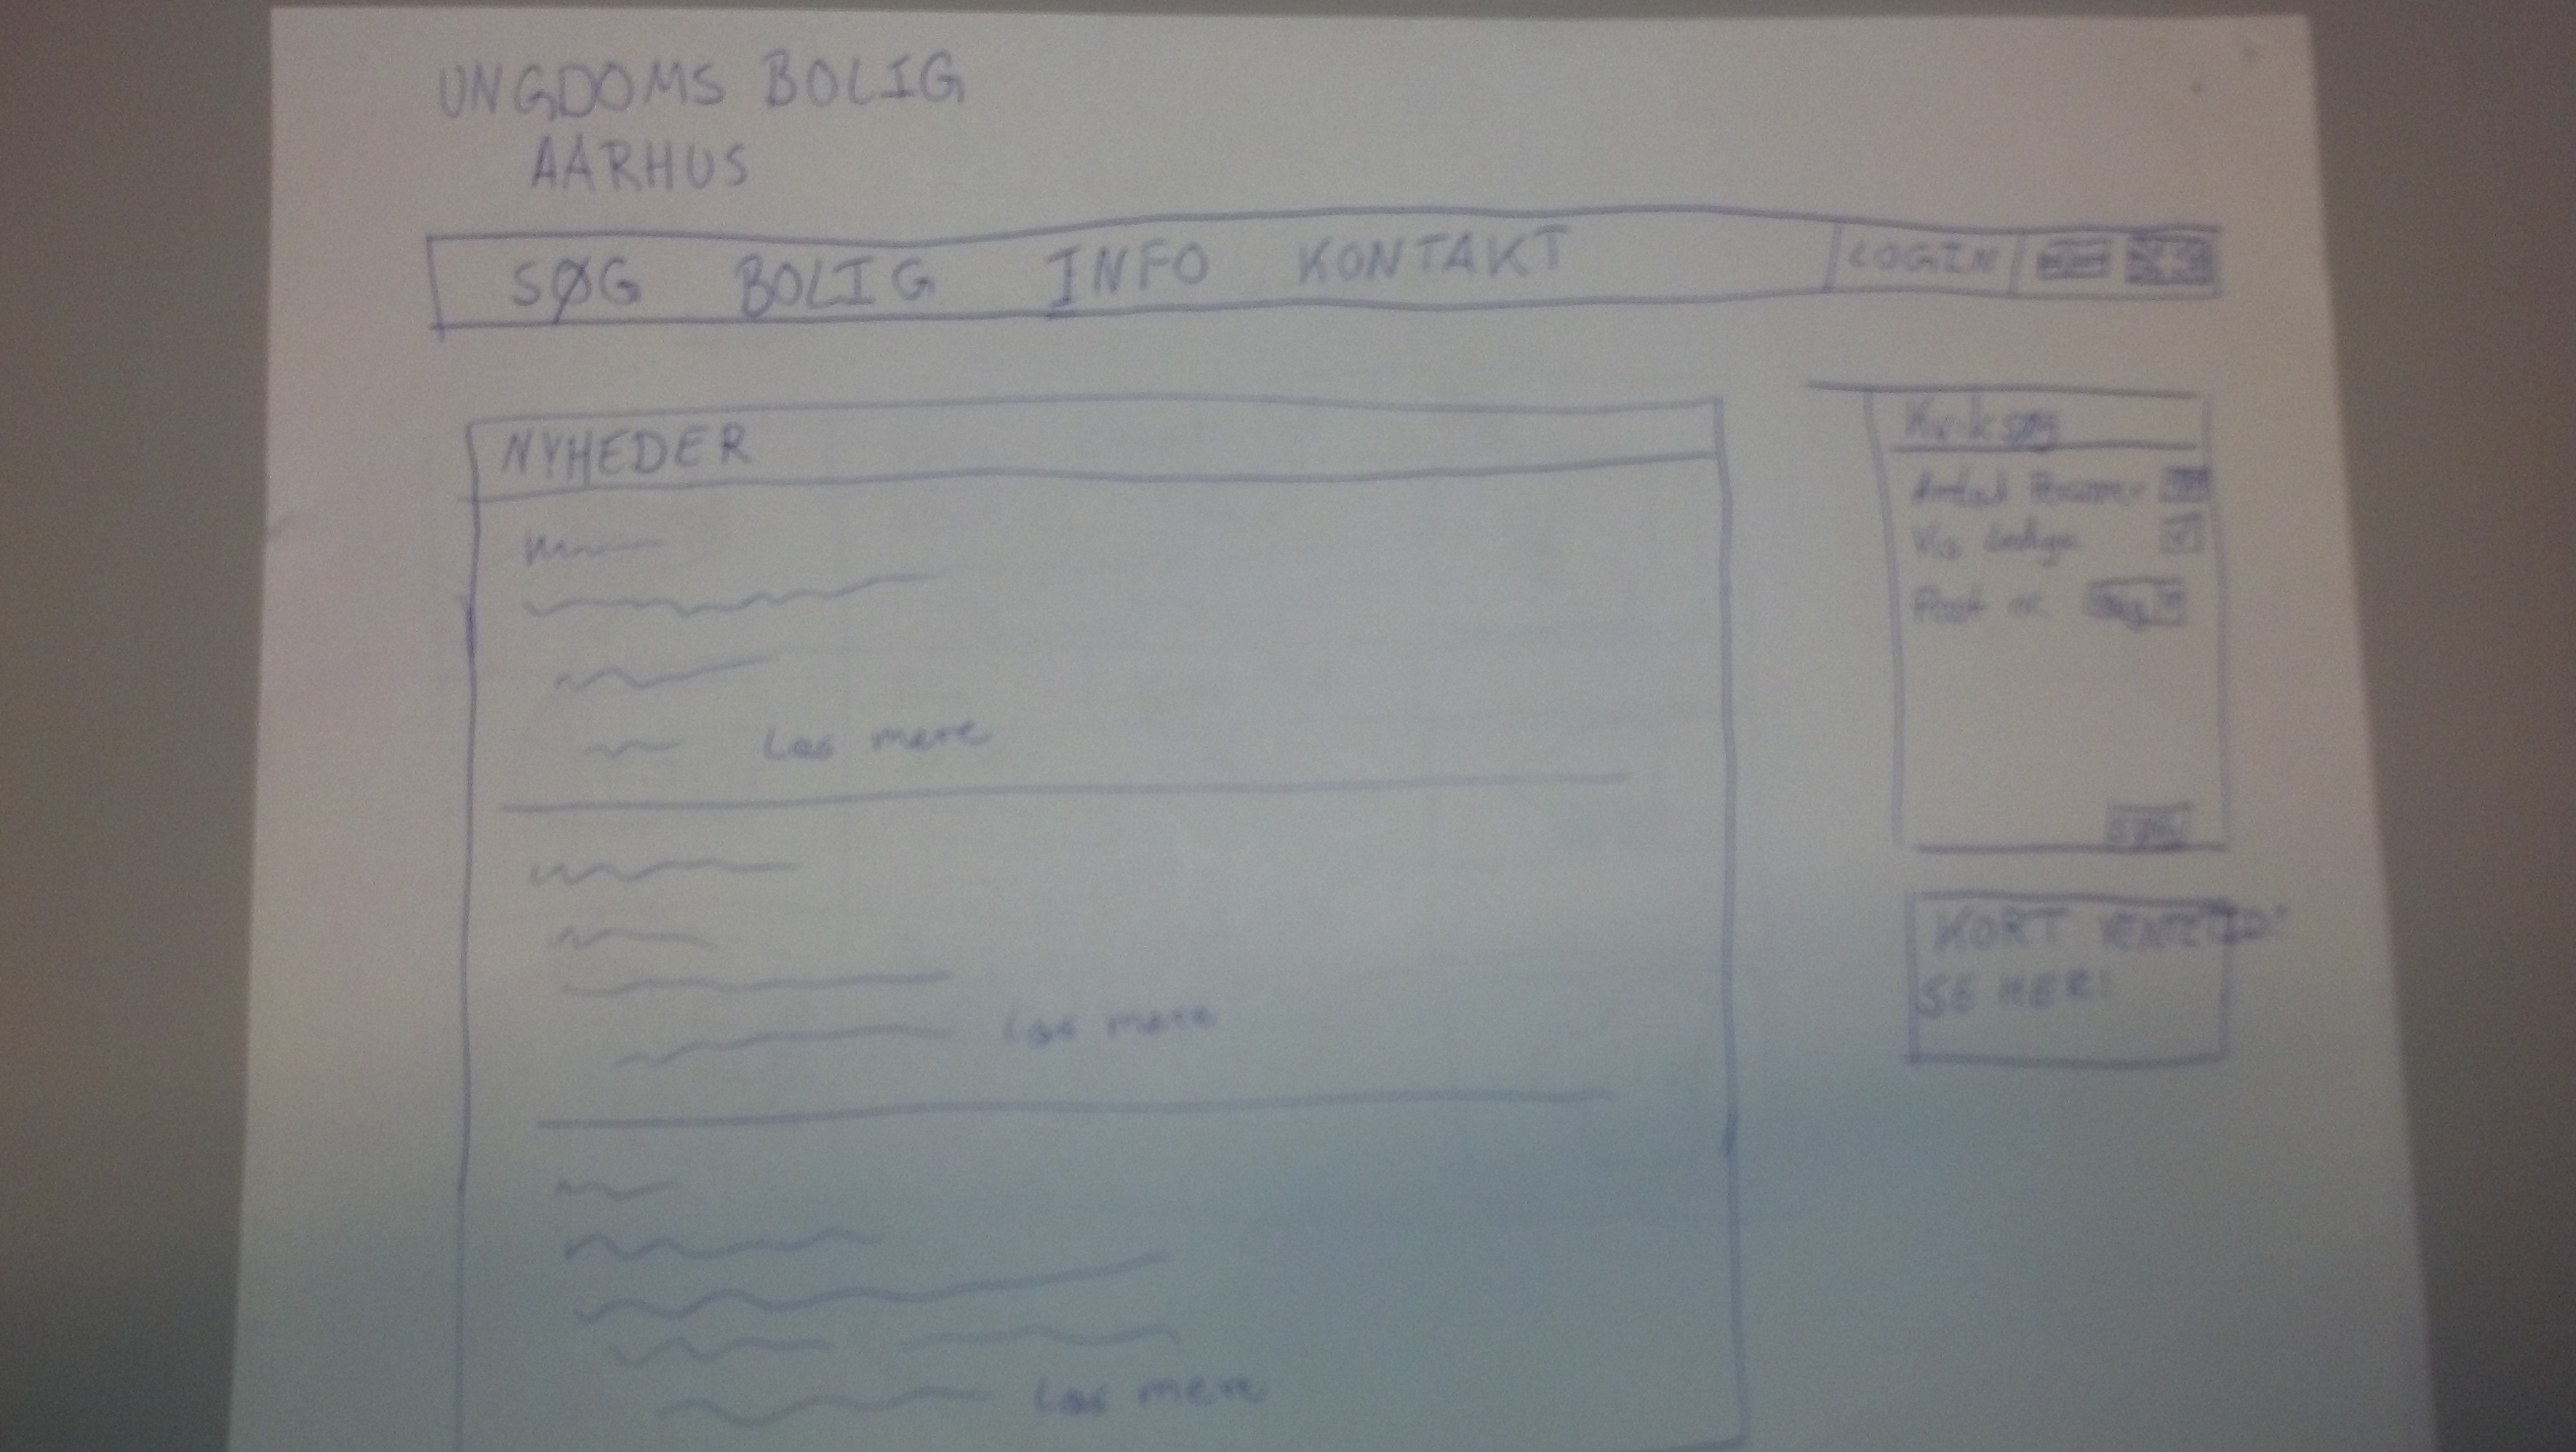
\includegraphics[width=0.5\textwidth]{eksperiment_forside}
\caption{Eksperiment: Forside med nyheder som hovedelementet, en simpel menu i toppen giver bedre overblik og navigation}
\label{e_forside}
\end{SCfigure}

\begin{SCfigure}
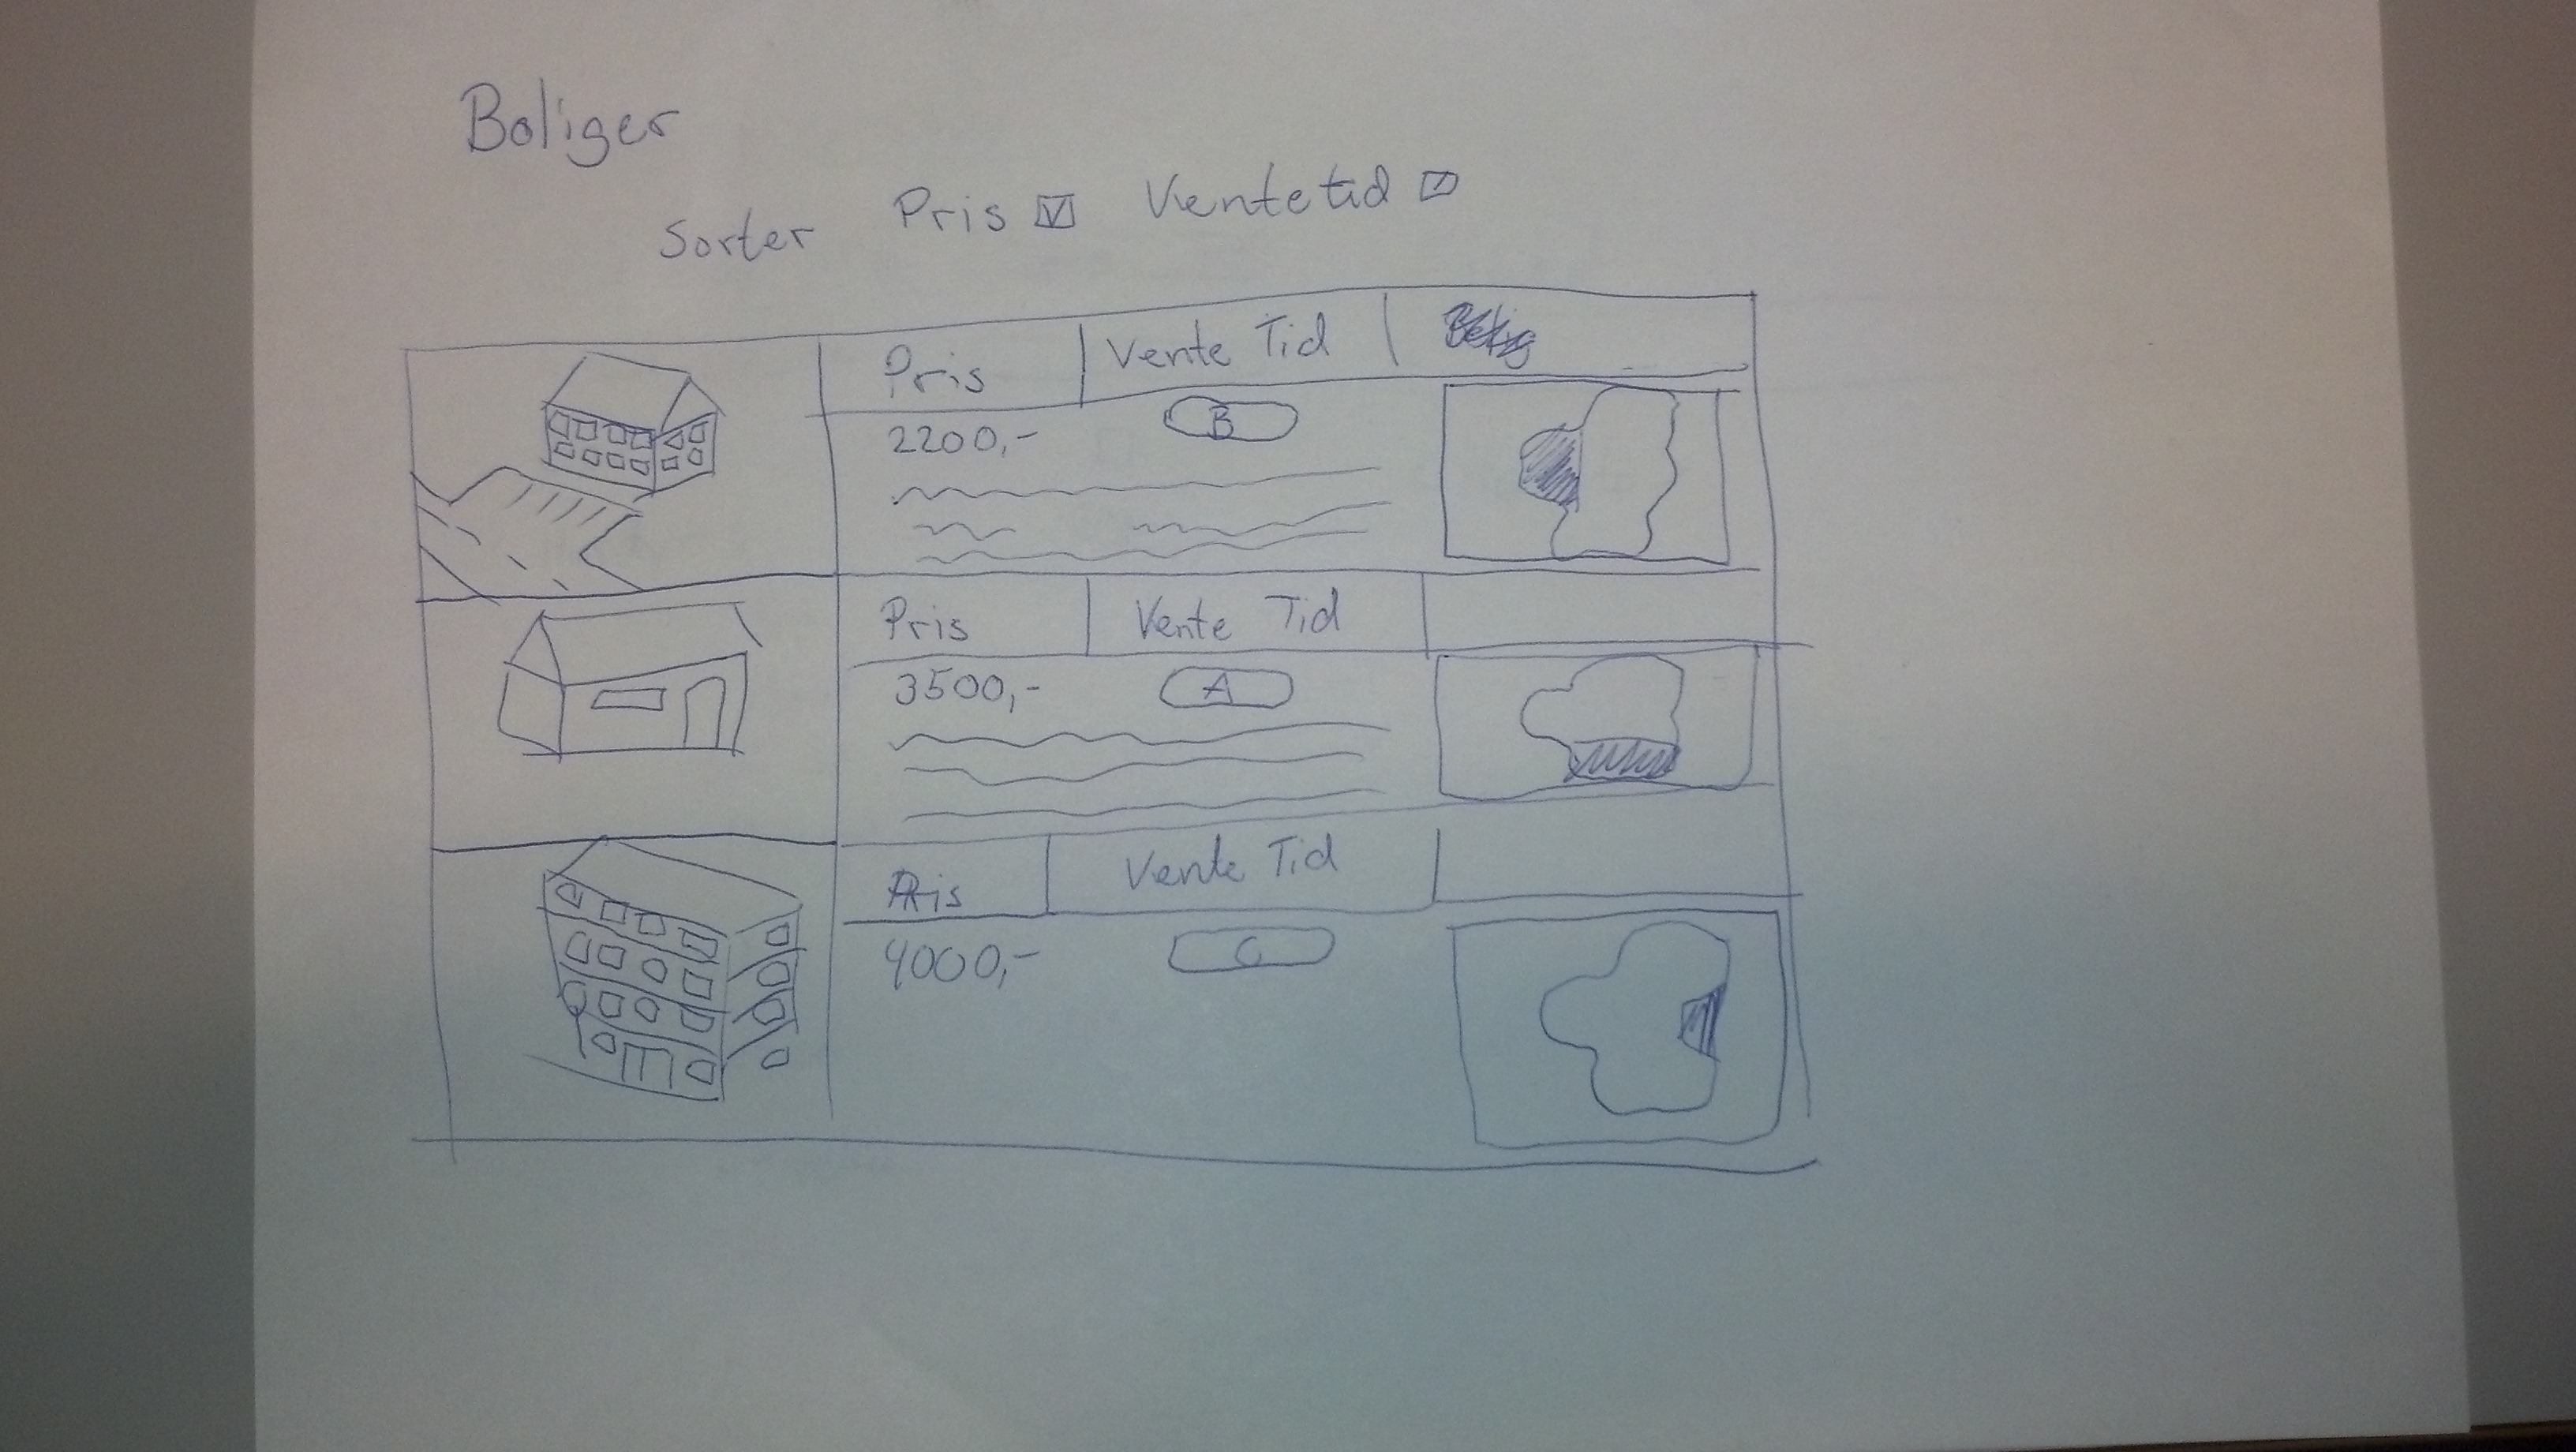
\includegraphics[width=0.5\textwidth]{eksperiment_liste}
\caption{Eksperiment: Liste / Søgeresultat med fokus på det værelse der passer til søgningen men stadig med data fra den afdeling det hører under}
\label{e_liste}
\end{SCfigure}

\begin{SCfigure}
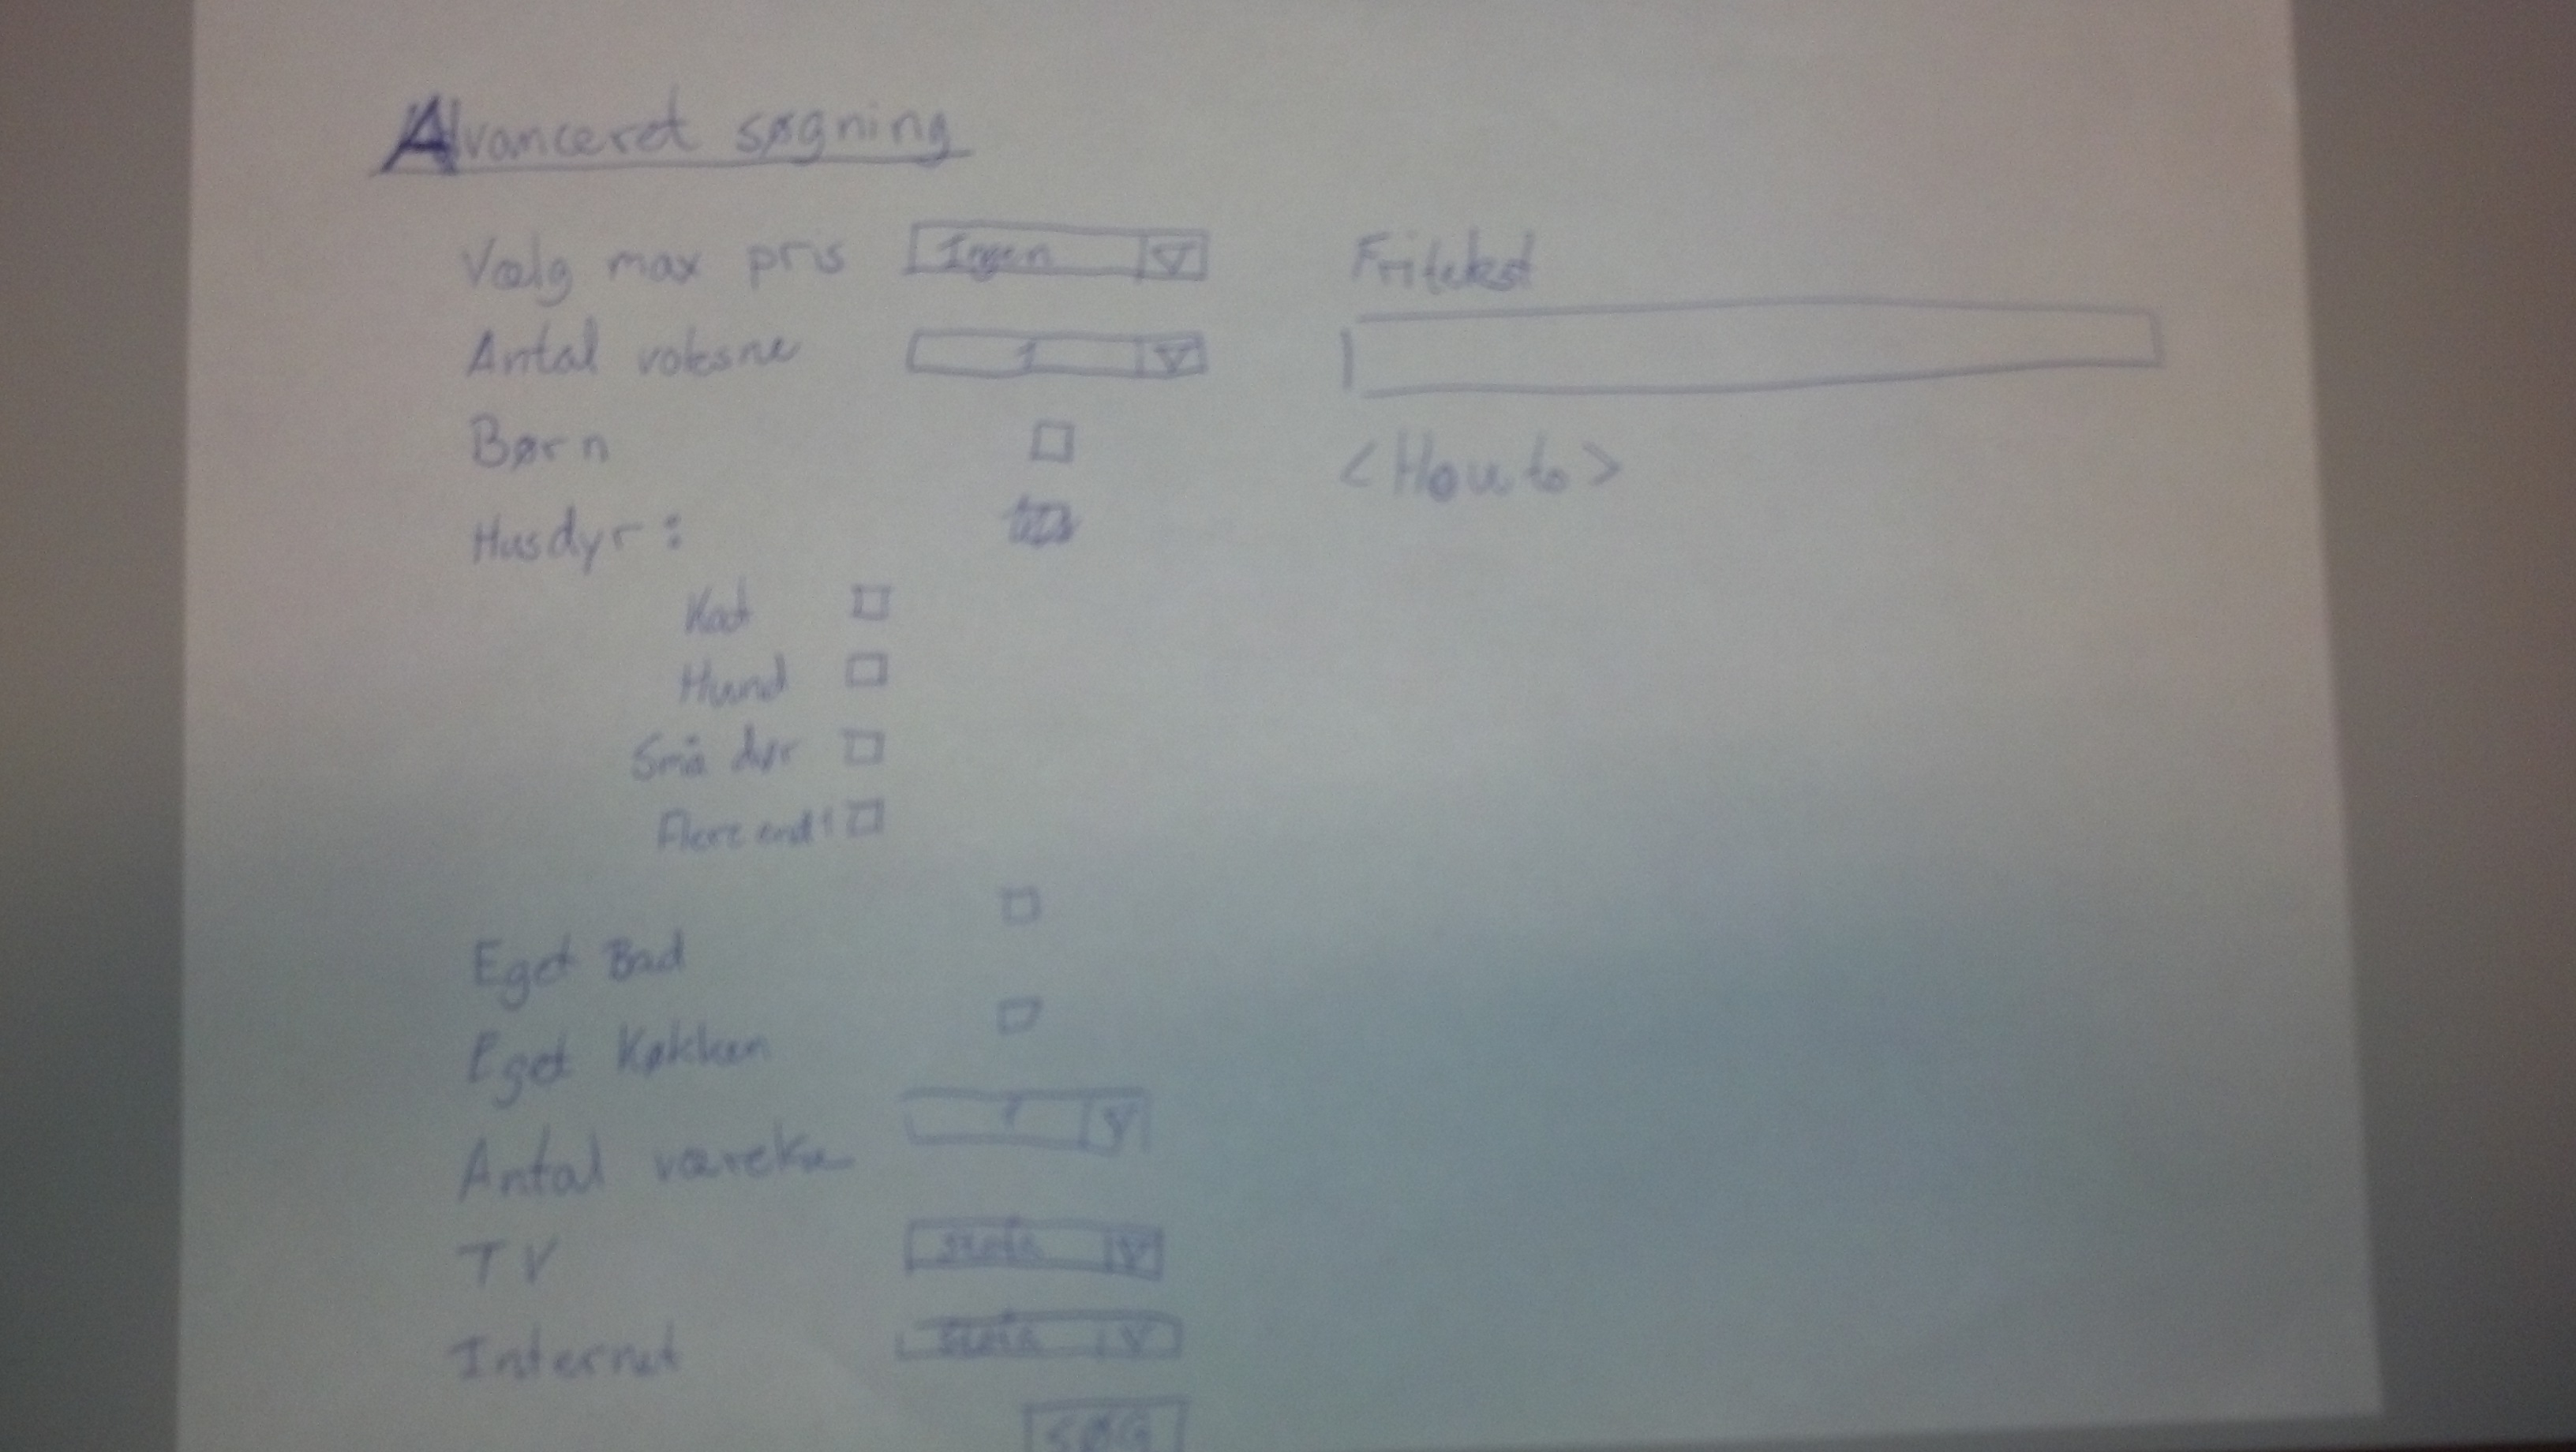
\includegraphics[width=0.5\textwidth]{eksperiment_soeg}
\caption{Eksperiment: Avanceret søgning. Overblik over de muligheder der kunne være i en avanceret og tilpasset søgning, layout vil blive optimeret.}
\label{e_soeg}
\end{SCfigure}

\end{document}

